%----------------------------------------------------------------------------------------
%	PACKAGES AND OTHER DOCUMENT CONFIGURATIONS
%----------------------------------------------------------------------------------------

% De documentclass 'article' is de beste voor bijna elke situatie.
\documentclass[a4paper,11pt]{article} % Default font size is 12pt, it can be changed here

% Packages:
\usepackage{geometry} % Required to change the page size to A4
%\usepackage[dutch]{babel} % Als je in het nederlands schrijft is dit nodig voor juiste afbreekregels en titels!
\usepackage{graphicx,xcolor} %colors and images
\usepackage{subfigure} %useful for multiple figures in one float
\usepackage{setspace} % iets met ruimte tussen regels
\usepackage{multicol} % meerdere kolommen
\usepackage{float} % Allows putting an [H] in \begin{figure} to specify the exact location of the figure
\usepackage{amsmath, amssymb}%Mathematical symbols
\usepackage[exponent-product=\cdot, per-mode=symbol]{siunitx} %Useful for physical quantities with units
\usepackage[notrig]{physics} %contains all kinds of useful abbreviations for braket, derivatives, etc.
\usepackage{enumitem,fancyhdr,lastpage,parskip} %For item lists, for headers and footers and no indents
\usepackage[numbers,square,super,sort&compress]{natbib} %For a bibliography
\usepackage[hidelinks]{hyperref}
\usepackage{listings} %Listings package is for scripts
\usepackage{cprotect} %For verbatim code in title...
\allowdisplaybreaks

% CODE ENVIRONMENT
\definecolor{mygreen}{rgb}{0,0.6,0} \definecolor{mygray}{rgb}{0.5,0.5,0.5} \definecolor{mymauve}{rgb}{0.58,0,0.82}
\lstset{basicstyle=\footnotesize, breakatwhitespace=false, breaklines=true, commentstyle=\color{mygreen}, extendedchars=true, frame=single, keepspaces=true, keywordstyle=\color{blue}, language=Python, numbers=left, numbersep=5pt, numberstyle=\tiny\color{mygray},  rulecolor=\color{black}, showspaces=false, showstringspaces=false, showtabs=false, stringstyle=\color{mymauve}, tabsize=3, title=\lstname, captionpos=b}
\setlength{\headheight}{27.85004pt}
%See for comments for instance here: https://tex.stackexchange.com/questions/83882/how-to-highlight-python-syntax-in-latex-listings-lstinputlistings-command

%%% SET HEADER/FOOTER
\pagestyle{fancy}
\fancyhf{}
\rhead{Krystian Czerniak (s3289451)\\ Thorben Plugge (s2938111)}
\lhead{Measuring nm vibrations \\with interferometry}
\cfoot{\thepage\ of \pageref*{LastPage}}

\begin{document}

\textbf{Measuring nanometer vibrations with interferometry} \newline
Krystian Czerniak s3289451 \newline
Thorben Plugge s2938111 \newline
Physics Experiments 3 Group A \newline 
27.03.2023 \newline
Dr. Paul Logman

\section{Introduction} 
Everything in our world vibrates, from small molecules to huge skyscrapers. Sometimes it is desired, like in our headphones, but sometimes it is an undesired byproduct that disturbes our machinery. Measuring nanometer vibrations would enable us to measure and correct for even these miniscule vibrations and probe further into the realm of the atoms with our new microscopes, like STM or AFM. This would not only help the scientific community, as accurately measuring vibrations lays at the foundation of many modern field, this could be very beneficial to the day to day life of regular people as well. Understanding vibrations can tell us much about the properties of materials, behaviour of atomic particles, and so much more that can and has been applied in the technology that we deem normal. In our research, we will look at how accurately we can measure vibrations such as these with interferometry. 

%----------------------------------------------------------------------------------------------------------

\subsection{Theory}
We will measure vibrations using interferometry. This is nothing unheard of since even the LIGO, the gravity waves detector, is in essence a Michelson and Fabry-Perrot inferometer, which is able to measure strains/vibrations in scale of $10^{-21}$\cite{Review}! 

We will use the classic approach though, the original Michelson-Morley interferometer \cite{original}. That is an interferometer that works using a laser of a specific frequency, a beamsplitter, two mirrors, and a detector. The laser is send through the beamsplitter where it is split into two and send towards two mirrors. These mirrors are ideally positioned at the same distance, so that when the beams hit the mirrors, bounce back, and recombine on the other side of the beamsplitter when hitting the detector, destructive interference should happen. But in the real world, due to the non-ideal coherence of the laser beam an bulls-eye interference pattern is visible, with a dark central spot.

We will sligthly tweak the classical design by placing an oscillating mirror at the end of one arm. The oscillation will cause a path difference between the arms given by $\Delta d = 2d_{1} - 2d_{2}$, where $d_1$ and $d_2$ are the lengths of the two arms. It is the same mechanism as in LIGO and what Michelson thought would happen due to the aether. The intensity of the central dot will then change, as in the formula below, and from that intensity we can read the frequency and the maximal amplitude of the oscillation.

\begin{equation}
S = P_0 * \cos^2(2\pi \Delta d/\lambda)
\end{equation}
Formula 1: A formula for the intensity of the central dot S as a function of the path difference $\Delta d$ between the arms. $P_0$ is the intensity of the laser and $\lambda$ the wavelength. Note that $2\pi \Delta d/\lambda$ is the phase difference between the EM-waves in these two arms. The source is Bond et al., eq. 5.12 \cite{Review} 

According to Bond et al., section 5.3\cite{Review}, the intefrometer is most accurate when it is set to the "dark fringe". That is when the mirrors are set to destructively interfere at rest, i.e. the original setup with a phase difference of 90 or 270 degrees.

One problem we may run into is an aliasing-like effect. When phase difference would be greater than $2\pi$, that would not be noticed. We think that we may bypass it if we can identify discontinuities in the signal, which would be the points where mirror turns, giving us again the fequencies and maximal amplitudes.


%----------------------------------------------------------------------------------------------------------

\subsection{Research Questions}
\paragraph{Main research question} What is the highest SNR we can get for our interferometry vibrationmeter? 

\paragraph{Main hypothesis} We think that the highest SNR we can get is 2 with a confidence interval of 5\%, defined by us. We hope to get it higher and will aim for it throughout, but given the ease noise creeps in our setup we realistically expect 2 or less (see \ref{study}).

\paragraph{Sub question 1} What is the relation between the voltage sent to the piezo and the displacement of the mirror glued to the piezo?

\paragraph{Sub hypothesis 1} We expect the relation to be linear, since the displacement is small, thus the hystoresis loop can be approximated as linear, see figure \ref{Fig4}

\paragraph{Sub question 2} Is there a relation between the arm length of the interferometer and the SNR ?

\paragraph{Sub hypothesis 2} We expect that there is no relation between the arm length and the SNR in our distance scales of centimeters, given it is the length difference that results in the interference.

\paragraph{Sub question 3} How much we can improve the SNR by using techniques such as isolating the interferometer from outside vibrations, taking longer and repeated measurements, and using filters?

\paragraph{Sub hypothesis 3} We expect the SNR to improve by an order of magnitude when isolating it from outside vibrations. The noise coming from mechanical vibrations should at least partially be fixed using mechanical filters. This combined should improve the SNR 10 fold. We expect the gain for other techniques such as repeated measurements and filter to be marginal in comparison to the gain in SNR due to isolation, likely not much more than a 5\% increase.

%----------------------------------------------------------------------------------------------------------

\section{Methods subquestion 1}

\subsection{Setup}

To test the functionality of the most important components of our experiment we will use the setup as shown in figure \ref{Fig1}.

\begin{figure}[H]\label{Fig1}
  \centering
  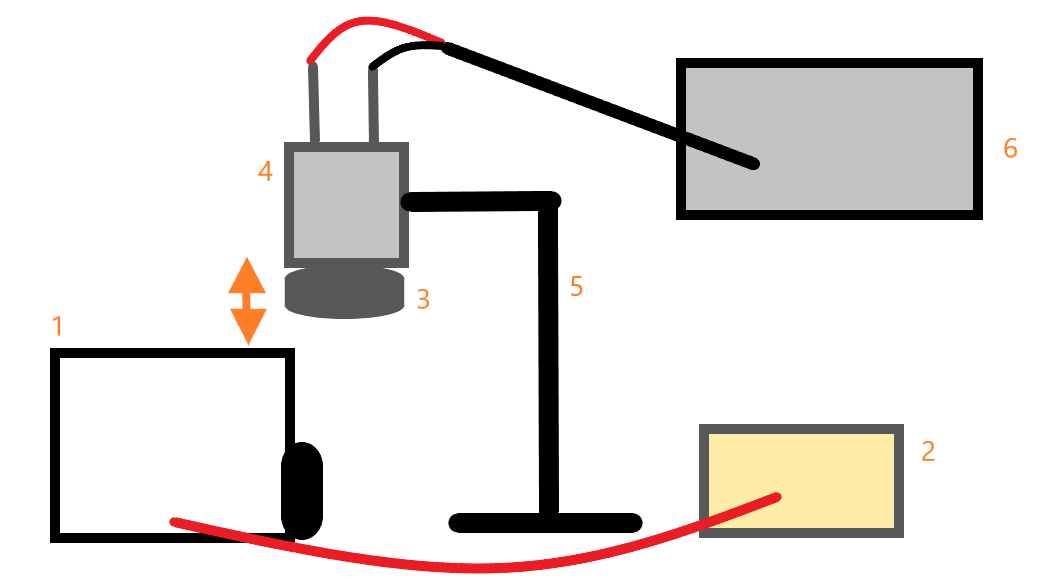
\includegraphics[width=0.9\textwidth]{tros.png}
  \caption{A schematic view of our setup, where we measure the relation between the incoming voltage and amplitude of vibrations due to the piezo.} 
\end{figure}

With Siglent function genetrator (6) a voltage will be sent to the piezo transducer (4) on a stand (5). Piezo will make the magnet (3) oscillate and that will cause a voltage in the GMR-sensor (1), which will be then sent to the multimeter (2). Precise distances between the components follow in the measurement method.

\subsection{Measurement method}

First, we will position the GMR sensor, such that the vertitical distance is $\SI{1}{cm}$ and the horizontal distance is $\SI{0}{cm}$, though we might deviate from these if other distances would give more accurate measurements. We will quickly measure that by moving the GMR-sensor in steps of $\SI{5}{mm}$ in both directions, lower and higher, and measuring the voltage with the multimeter. The piezo will be off during these measurements. The distance with biggest voltage, but in the linear region of the GMR (see fig \ref{Fig3}), will be chosen as the final distance.


Then we have to measure the magnetic field of the magnet. That may be already given in the specs, or we might measure it with the GMR or with a gaussmeter. 


It naturally depends on the piezo we will get, but we plan to vary the voltage over the piezo in steps of $\SI{0.5}{V}$, starting from $\SI{0}{V}$ and ending with $\SI{10}{V}$. These voltages should be well within the linear region of the hystoresis loop (see fig \ref{Fig5}). At each voltage we will do 10 separate measurements. As the output, we will also measure the voltage, but now over the GMR-sensor. Raw data errors will be determined with the null-measurement at $\SI{0}{V}$, to identify the errors, such as the systematic error due to the magnetic field of the earth, the thermal noise and EM-noise due to signals in unshielded cables. To counter the EM-noise and magnetic field, we might shield the unshielded cables as well as the whole setup with aluminum foil.

\subsection{Analysis method}

Given the voltage array from the GMR with a certain voltage in piezo, and the magnetic strength of the magnet, we can calculate the distance between the magnet and the sensor using a gauge sheet of the GMR-sensor, given in the appendix as the figure \ref{Fig3} and the fact that a magnetic dipole (approximation for our magnet) decreases with distance cubed.
\newline
That will be done for each measurement at certain voltage in the piezo and then they will be combined by taking the mean and standard deviation. The results at certain voltages will be the mean and the error will be the root-mean-square of the standard deviation and the error of the null measurement, given by the square root of the area of the FFT of the null measurements. These results will be then plotted in a graph and a fit will be performed to determine if the relation is linear or not. We will reject our hypothesis is the correlation between the fit and data is lower than 0.9, a reasonable reliability bound.

%----------------------------------------------------------------------------------------------------------

\section{Methods subquestion 2}

\subsection{Setup}

We are going to build two interferomters for this subquestion, one with long arms ($\SI{15}{cm}$) and the other with short arms ($\SI{5.5}{cm}$). Other lengths may be build if nessecary. Both will be build according to the setup on the figure 2.

\begin{figure}[H]\label{Fig2}
  \centering
  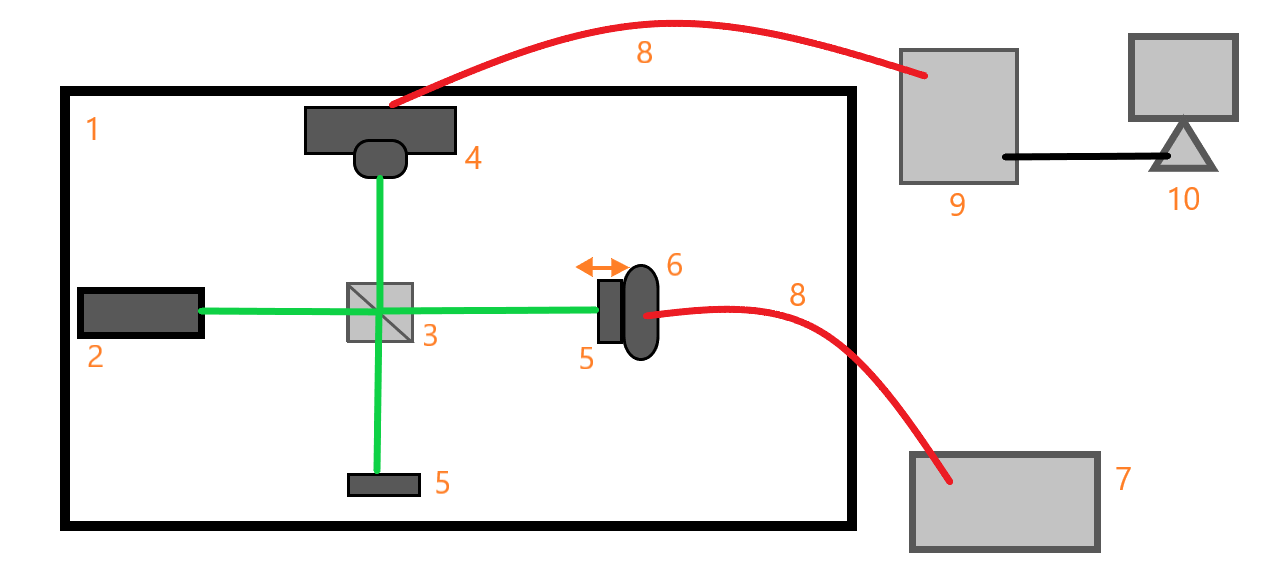
\includegraphics[width=0.9\textwidth]{sop.png}
  \caption{A schematic view of our setup, where we build a Michelson interferometer with one variable distance arm.} 
\end{figure}

Everything will be build on a optical breadboard (1). There we will screw a green light ($\sim \SI{500}{nm}$ wavelength) laser (2), 50-50 reflection beamsplitter (3), a photodetector (4), highly reflective ($>95\%$) mirrors, where one is glued onto a piezo transducer (6). The piezo is connected through a coax cable (8) to a function generator (7). The photodiode (4) is connected to a NI MyDAQ (9), which sends data to the computer (10).

\subsection{Measurement method}

To do the measurements, we will have to simply turn the laser on and start the automated measurement on the MyDAQ. During the measurement, we will leave the room and close it, so we don't disturb it. We will send a $\SI{40}{kHz}$ sine wave with an amplitude corresponding to $\SI{300}{nm}$ displacement to the piezo. The displacement has been chosen such it is smaller than the wavelength and no "alliasing" happens. The frequency has been chosen such it does not overlap with expected frequency of the noise (see feasibility study \ref{study}). Each measurement will be 30 seconds long and repeated 10 times. This will be done for both interferometers. As output we will receive voltage array in time from the photodetector. A null measurement will also be performed, where the piezo won't be oscillating to determine the noise. It will also be done 10 times, each 30 seconds long. This is neccesary to determine the errors due to outside light and vibrations. This procedure will be done for both distances.

\subsection{Analysis method}

Since the voltage from the detector is proportional to the intensity, we will work directly with voltages. To calculate the frequency of the vibration, we will use the FFT on the collected voltage data. To determine if our hypothesis is true, we will calculate the SNR for both distances and calculate the relative difference between them. If it is bigger than 5\%, then our hypothesis will be rejected. 

The SNR will be calculated by dividing the signal power by the noise power. First will be calculated by calculating the mean of the signal squared and then taking the mean of these 10 results. The std of that shall give the error in the power of the signal. Former will be calculated by calculating the FFT and calculating the area of that FFT and then taking the mean of these 10 results. The std shall again give the error.

%----------------------------------------------------------------------------------------------------------

\section{Methods subquestion 3}

\subsection{Setup}
We will use the same setup as in subquestion 1 (figure \ref{Fig1}), but this time in various stages of isolation and noise reduction. One setup is exactly as shown in subquestion 1, one is isolated in a sound isolation box, one is mounted on mechanical filters, and the last one is mounted on a mechanical filter inside an sound isolation box. These are barely any different from our original setup. Longer and repeated measurements will be done using the setup that reduces noise the most, but a filter will be added directly behind the detector of the setup when testing for SNR increases using a filter.

\subsection{Measurement method}
First we will measure with no dampening to establish a baseline. We will measure for 30 seconds 10 times to create enough of a log, before moving on to the dampening methods, where we will vary these techniques. We will measure the setup for the same time and number of measurements in sound isolation, before moving on to vibration dampening using mechanical filters on which we put the setup. We measure each seperately before combining the sound isolation and mechanical filter methods. The precise settings are the same as in subquestion 2 and different null measurements will be made for each variation in the setup, with the same time lengths and repeats.

Using this setup we will then use several noise reduction strategies seperately.

We will attempt to use three separate types of noise reduction: We will use a low-pass filter to eliminate all the very high frequency noise from the detector, we measure for much longer to average over a longer period of time and also average out the high frequency noise, and we will repeat the measurement several fold to get more trustful statistic. For first we will measure for 30 seconds 10 times with the filter, then for 1 minute 10 times to test a longer measurement time, and lastly for 30 seconds 20 times to test more measurements.

\subsection{Analysis method}
When we have all the 10 datapoints from each of the sound and mechanical filter setups, we will calculate the SNR like in the previous subquestion. We expect the combination of sound and mechanical filters to be the most effective, and hope to achieve a SNR ratio increase of $\sim 10$, and hope that the signal of our vibration is clearly visible over the noise. We will use the described techniques of longer measurements as well as repeated measurements to lower this SNR even further, although we will do this several times to avoid outliers playing too large a part. We will compare each technique using this calculated SNR, compare them to our hypothesis in order to verify it, and choose our final setup based on the highest one.

%----------------------------------------------------------------------------------------------------------

\section{Main Methods}

\subsection{Setup}
Using the techniques we found work best in the previous subquestions we set up for the final measurements. This will likely be a combination of the setup in subquestion 1 (figure \ref{Fig1}) and additional techniques from subquestion 3.

\subsection{Measurement method}
Using a complete setup determined by the combination of our sub conclusions we can start measurements for the main research question. We expect to find that mechanically and sonically isolating the setup will improve the SNR, so the measurements will be done in a soundproof box on a mechanical filter. 

Additionally, we expect that measuring longer and with more repetitions will improve the SNR, and so we will measure for as often and as long as sub question 3 indicates gives the best returns. Although we cannot definitively predict how much time this will take, we assume that we will repeat the measurements dozens of times at minimum, and hope to take several hours to complete these measurements.

We will measure the same observables we measured during subquestion 2: the voltage over de detector. This is directly proportional to the intensity of the pattern that falls on the detector. We will send in a $\SI{40}{kHz}$ sine wave with an amplitude that corresponds to a $\SI{300}{nm}$ displacement of the piezo, like in the subquestion 2 with the same reasons.

\subsection{Analysis method}
Like in previous subquestions, from our voltage array we will calculate the frequency, maximal displacement and the SNR, like described in the theory and the previous subquestions. The SNR will be our main point of interest, and using the techniques we've discovered work best in the previous sub questions we will reduce noise as much as possible. This is done mostly during the measurements (repeating them, for instance) but a few things can be done to reduce noise during analysis. We will calculate the noise through the standard deviation of our repeated measurements, and using electronic analysis will reduce human error. 

Then, using this final SNR, we will compare it to our hypothesis. If it differs by more than 5\%, we will reject our hypothesis.

%----------------------------------------------------------------------------------------
\section{Sub question 1 measurements}
\paragraph{18-04-2023 09:41} 

%----------------------------------------------------------------------------------------
%	BIBLIOGRAPHY
%----------------------------------------------------------------------------------------
\section{Task-risk analysis}

\begin{figure}[H]\label{TRA}
  \centering
  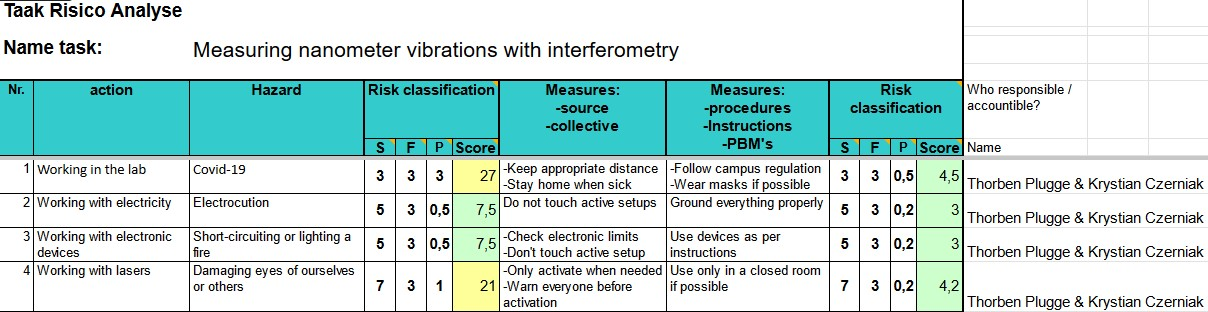
\includegraphics[width=0.9\textwidth]{TRA.jpg}
  \caption{The task-risk analysis of our experiment.} 
\end{figure}

\section{Appendix}

\subsection{Feasibility study}\label{study}

The vibrations due to the outside noise should couple very weakly, because the lab building is quite sturdy. To support our claim, we refer to figure \ref{Fig6}. In the bachelor lab, we can't feel any vibrations if no humans are around. That means the vibrations must be at most in the order of $\SI{1}{\mu m}$, if we assume that a noise vibration decomposes equally in all frequencies. That would give a SNR of $\sim 0.3$ at worst, given our vibrations are in range $\SI{0.3}{\mu m}$. With use of mechanical filters, we will reduce all high-frequency noise and 60\% at $\SI{20}{Hz}$. Low-frequency ($<\SI{15}{Hz}$) noise is hardly damped by the mechanical filters. We think then that with all techniques described above we could reach a SNR of 1 and in best case 2.

\subsection{Additional figures}

\begin{figure}[H]\label{Fig3}
  \centering
  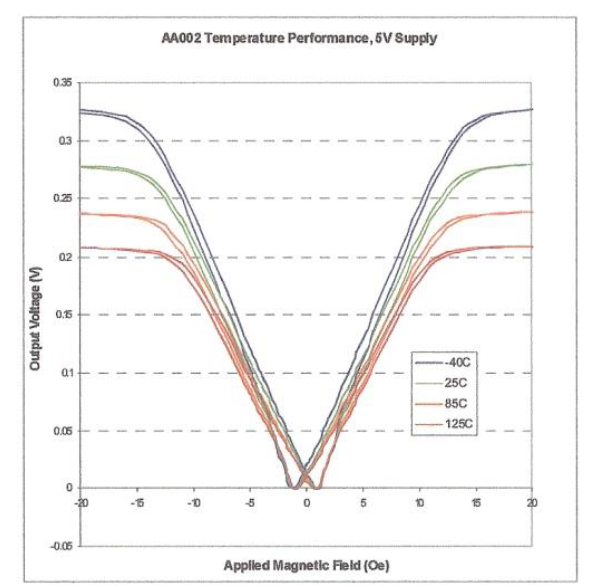
\includegraphics[width=0.9\textwidth]{ijk GMR.png}
  \caption{The guage sheet of the GMR-sensor availible in the lab. Note that the relation between the voltage and magnetic field is nearly linear with saturation above ~10 Oe.} 
\end{figure}

\begin{figure}[H]\label{Fig4}
  \centering
  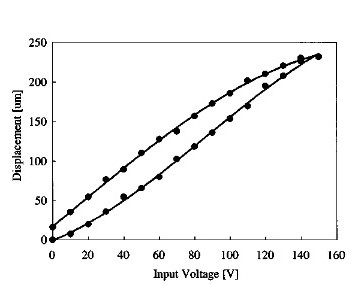
\includegraphics[width=0.9\textwidth]{guage.jpg}
  \caption{A gauge sheet of a piezoelectric actuator. Clear hystoresis loop can be seen as the relation between the displcement and the voltage. Precise values may differ for each different piezomodel, for example there are piezo which operate in the nm or mm region with same voltages. The precise values may also depend on the frequency, see figure \ref{Fig5}. The source of this graph is Morita et al.\cite{guage}} 
\end{figure}

\begin{figure}[H]\label{Fig5}
  \centering
  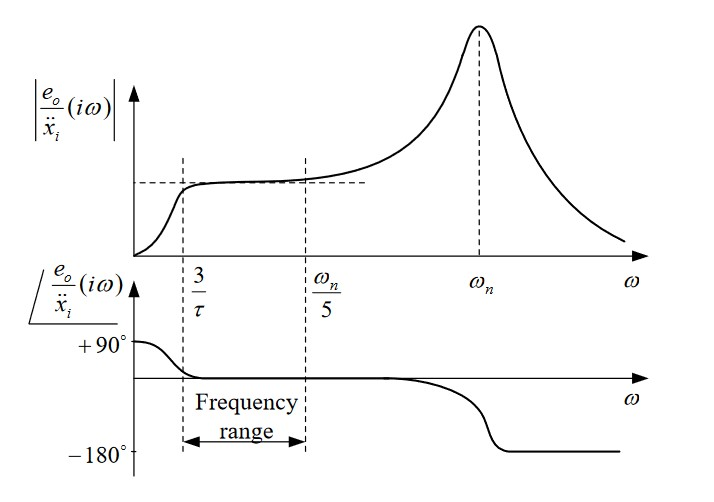
\includegraphics[width=0.9\textwidth]{freq.jpg}
  \caption{The frequency response of a typical piezoelectric transducer. It can be modelled as a high-pass coupled with a low-pass resonant filter. The precise values depend on the model. The source of this figure is Yu and Lan \cite{freq}} 
\end{figure}

\begin{figure}[H]\label{Fig6}
  \centering
  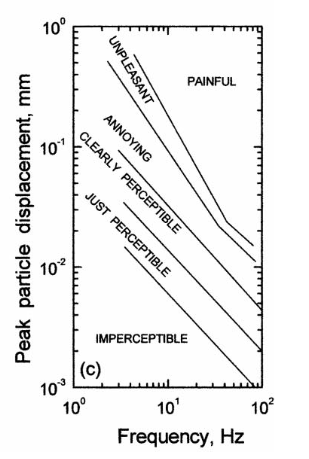
\includegraphics[width=0.9\textwidth]{vibes.PNG}
  \caption{A graph showing human perception of the vibrations. The source is Athanasopoulos et al., figure 7\cite{vibes}} 
\end{figure}

\addcontentsline{toc}{subsection}{References}
\begin{thebibliography}{99} % Bibliography - this is intentionally simple in this template
\bibitem{guage}
Morita, T., Shimizu, K., Hasegawa, M., Oka, K., \& Higuchi, T. (2002). A miniaturized levitation system with motion control using a piezoelectric actuator. IEEE Transactions on Control Systems and Technology. https://doi.org/10.1109/tcst.2002.801802 
\bibitem{freq}
Yu, J., \& Lan, C. (2001). System modeling of microaccelerometer using piezoelectric thin films. Sensors and Actuators A-Physical, 88(2), 178–186. https://doi.org/10.1016/s0924-4247(00)00502-1

\bibitem{original}
Michelson, A. A., \& Morley, E. W. (1887). On the relative motion of the Earth and the luminiferous ether. American Journal of Science, s3-34(203), 333–345. https://doi.org/10.2475/ajs.s3-34.203.333

\bibitem{Review}
Bond, C. Z., Brown, D. G., Freise, A., \& Strain, K. A. (2016c). Interferometer techniques for gravitational-wave detection. Living Reviews in Relativity, 19(1). https://doi.org/10.1007/s41114-016-0002-8

\bibitem{vibes}
Athanasopoulos, G., \& Pelekis, P. C. (2000). Ground vibrations from sheetpile driving in urban environment: measurements, analysis and effects on buildings and occupants. Soil Dynamics and Earthquake Engineering, 19(5), 371–387. https://doi.org/10.1016/s0267-7261(00)00008-7
\end{thebibliography}

\end{document}